

\section{Motivation for the Search Model}

\textbf{Big Picture}: the Rental market behaves much more like the labor market than it does the car market. Firms post vacancies, tenants apply, contracts are bargained over, and posted units may or may not actually be available to tenants. This matters for how we think about market power and modelling the housing market. \\

Right now, I'm working of of \cite{jarosh-search-2024}'s model of the labor market, adapted for the rental market. Ideally, I'd like to take the insights from this model, but adapt it to something closer to standard IO methods. Any insight onto how to do this is appreciated.\\

\textbf{Why this matters}: 
Up front, I wish I had some better reasons for why you need to consider search in this market, beyond the fact that I think search costs and outside options are what creates market power and that there's an interesting way in which landlords can avoid competing with themselves by influencing their tenants' outside options. What would be helpful would be if anyone has any thoughts on how to motivate the "why search" better.\\

Recent models of market power in housing market model the supply side with differentiated Bertrand competition (sometimes Cournot), where market power comes from product differentiation and quantity reduction. The first issue is that some implied elasticities from empirical estimates of prices and vacancies are not consistent with elasticities from demand estimation. The second issue is that, because most housing was built decades ago, firms can only move around quantities by:\\
\begin{enumerate}
    \item internalizing market power at time of development (unlikely for old buildings)
    \item moving around quantities by changing vacancy rates, in which case search is the natural way to think about the problem
\end{enumerate}


In particular, it's  likely that landlords flex monopoly power by exploiting search costs and influencing tenants' outside options. One simple example of this is that they can exploit tenant switching costs. In this hypothetical, a landlord would give a tenant an offer and threaten that, if they don't accept the offer, they won't be able to rent to any of the landlord's other units. Effectively, landlords need not compete with themselves.

% \section{Intuition}
% To fix intuition, consider two markets of 1000 homogenous units each. In market 1, there are 100 landlords who each lease 10 units. In market 2, there are 10 landlords leasing 100 units each. Standard competition models say that as long as their vacancy rates are the same, so will market prices. I think this is weird!

\subsection{Empirical Example}

Take this job market paper from this year. The first figure (\ref{fig:fern-prices}) is the results from a Diff in Diff on mergers of rental properties, filtered for mergers that increase concentration by a substantial amount. The second figure \ref{fig:fern-vacancies} plots the same regression but with the change in the number of vacant units as the dependent variable\\

She estimates prices effects in the order of 7.5\%. \footnote{You can square this result with my field paper that shows no effect of these kinds of mergers by noting that she filters for mergers that are in the top 5\% of changes in predicted concentration; likely the total ATT is zero} She then explains this by noting that firms also increase vacancies concurrently with hiking prices (and that it doesn't look like they're doing unobserved quality upgrading). However, she finds vacancy effects in the order of a 5-10\% decline in \textit{own supply}. This would imply own price elasticities of around -0.66 to -1.3, some of which would be on the wrong part of the demand curve, and all of which are inconsistent with what other people in the literature have found (median elasticities of around -3).

\begin{figure}[htbp]
        \centering
        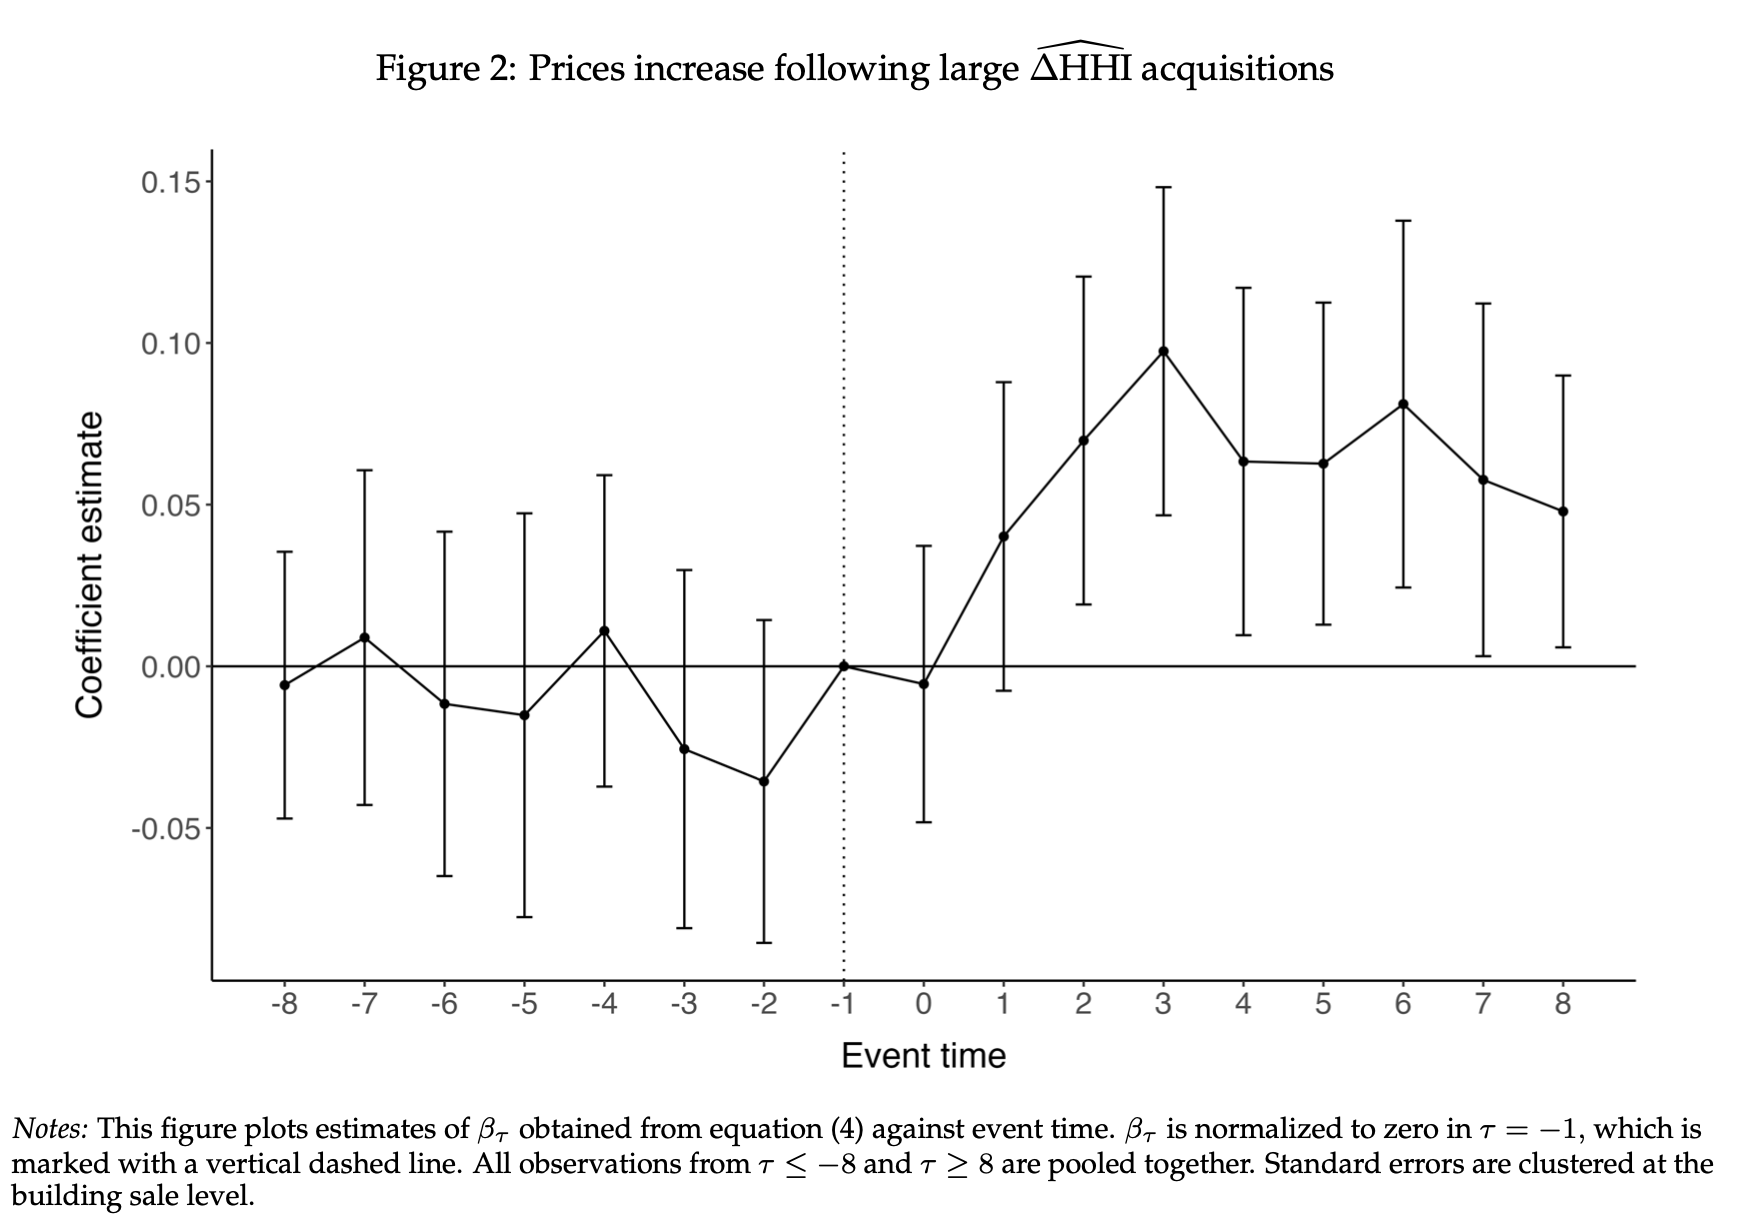
\includegraphics[width=0.5\linewidth]{figs/fern-jmp-prices.png}
        \caption{Effect of large merger on prices}
        \label{fig:fern-prices}
    \end{figure}

\begin{figure}[htbp]
        \centering
        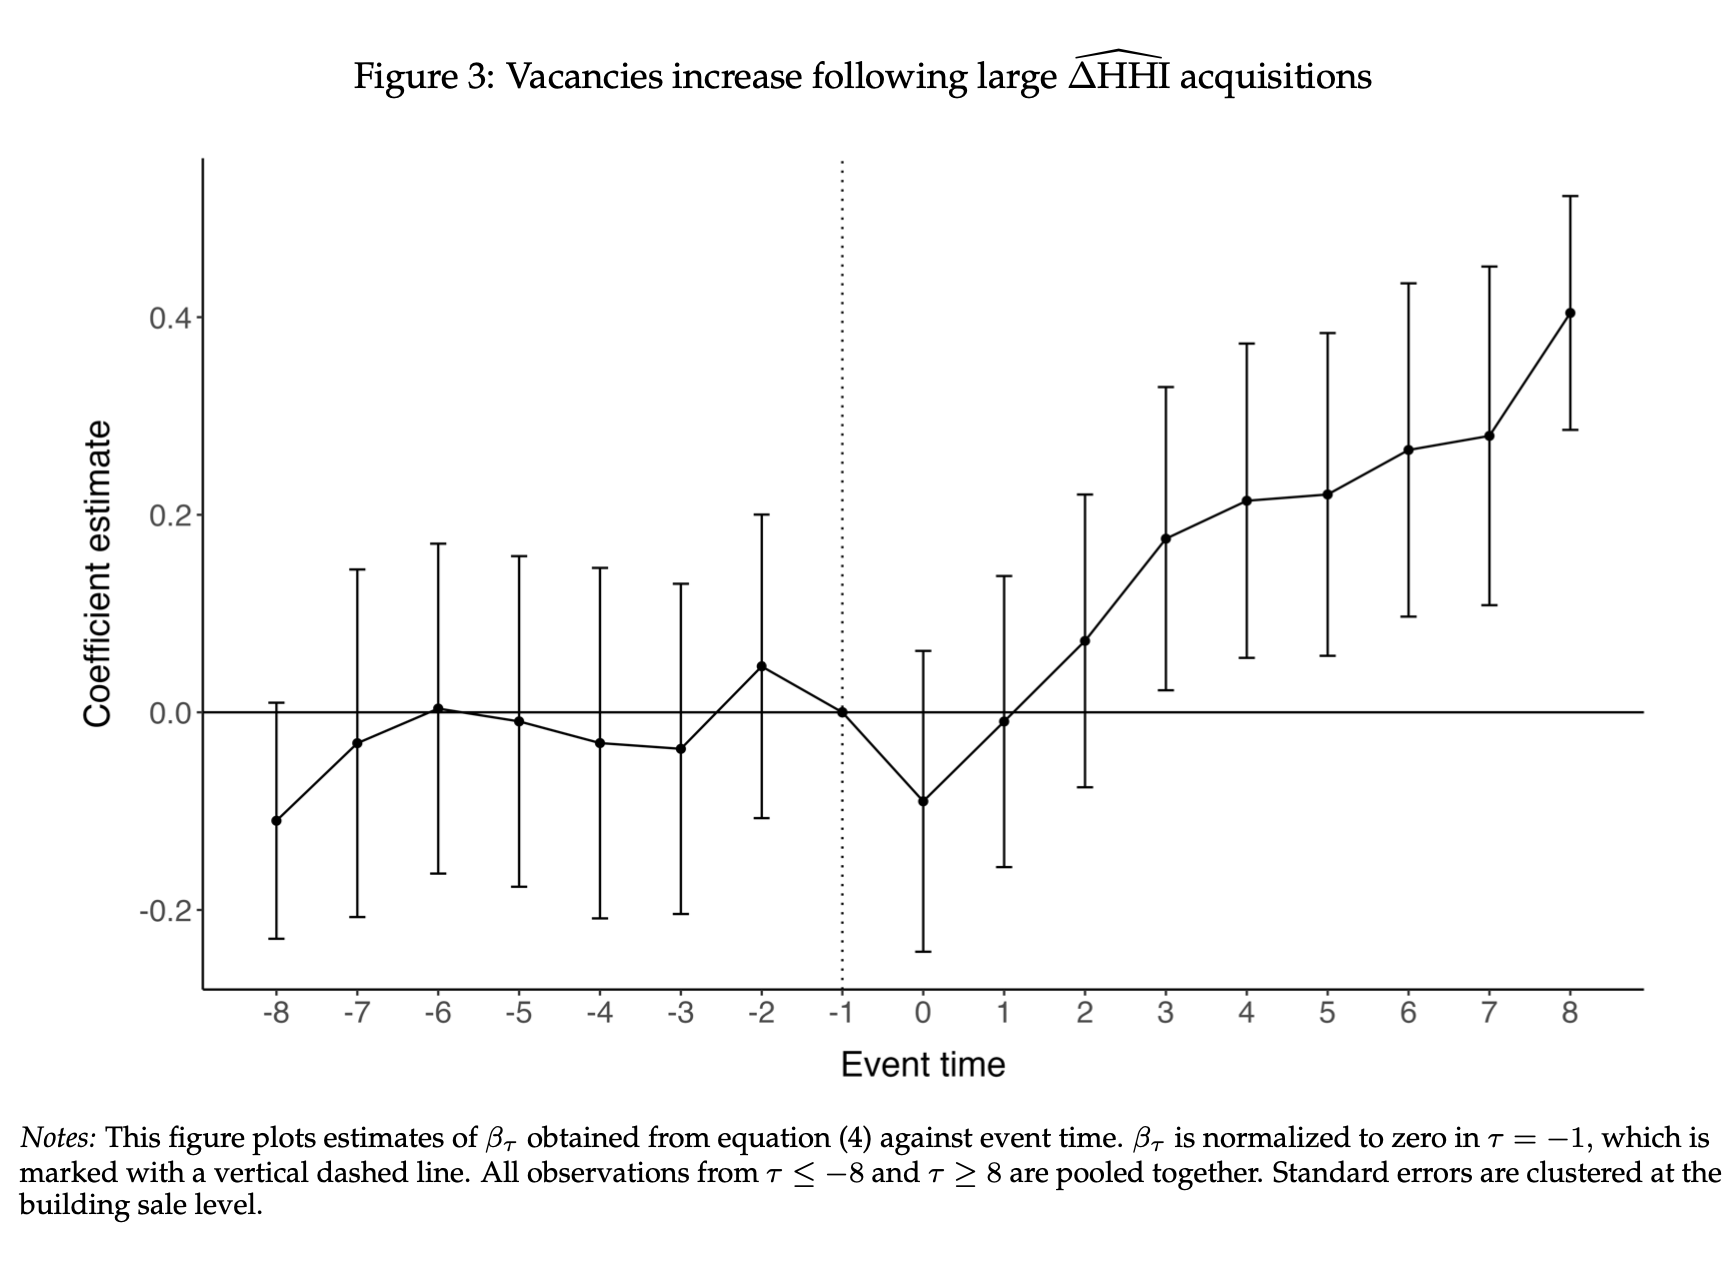
\includegraphics[width=0.5\linewidth]{figs/fern-jmp-vacancy.png}
        \caption{Effect of large merger on vacancies}
        \label{fig:fern-vacancies}
    \end{figure}

% \section{RealPage}
% RealPage is an example of where I think firms actually are doing Bertrand style quantity reduction. However, I think this makes my point: with RealPage, market vacancy rates get reduced by ~3\% and prices go up by 3-5\%. This is a much more normal effect than what other people are finding.


\section{Model}

\subsection{Setup}

\begin{itemize}
    \item Discrete time economy
    \item Unit measure of infinitely lived, homogenous renters
    \item Renters are either housed and pay rent ($R$) to receive flow utility ( $\boldsymbol{\eta}$) or are unhoused / consuming some outside housing good \textbf{$u$} and searching while receiving flow utility \textbf{$b$}
    \item Common discount factor \textbf{$0 < \beta < 1$}
    \item Housed / non-searching renters experience exogenous separation shock at rate  $\boldsymbol{\delta}$
\end{itemize}

\subsection{Matching}
\cite{jarosh-search-2024} labor search model, adapted for the rental market 
    \begin{itemize}
        \item Standard search and matching model for labor
        \item Twist is that landlords can remove themselves from tenants' outside option
        \begin{itemize}
            \item Intuition is landlords can say "you can rent this unit, but if you refuse my offer, I won't show you any other units"
            \item This is costless in a world where vacancies see multiple applications
        \end{itemize}
        \item Model delivers market power without landlords having to reduce vacancies
    \end{itemize}

\subsection{Tenant Value Functions}

Let \textbf{U} = value of outside option (homelessness; living in non-preferred neighborhood), \textbf{R} = rent paid; \textbf{b} = flow utility of outside option, $\boldsymbol{\eta}$ = flow utility of housing, and $\boldsymbol{f_i}$ indicate the landlord size (market share). Then the tenant's value function is:

\begin{equation}
        U = b + \beta\left(\lambda \sum_{i} f_i(\eta - R_i) + (1-\lambda)U\right)\label{eq:tenant-val}
    \end{equation}\label{eq:tenant-val}

Here, the value of outside option is equal to flow utility plus probability of being housed in next period times the value of being housed plus the probability of remaining unhoused times the value of being unhoused.

\subsection{Threat and Market Power}

In eq \ref{eq:tenant-val}, firms compete with themselves because the firm's other vacancies enter the worker's outside option. What firms can do instead is (partially) remove themselves from the tenants' outside option by committing themselves to not renting to the tenant in the future in the event bargaining breaks down. This commitment works by firm's choosing applicants randomly but removing the tenant in the event they have multiple applicants. Importantly, this is costless to the firm, since they have multiple applicants. (If the deviating tenant is sole applicant, they get the unit)\\

 I say that this punishment lasts until the tenant's search is over, so landlords need only be able to recognize a tenant's application for a short period of time. Intuitively, one could imagine a property manager making an take it or leave it offer to a tenant with the threat that if they leave it they can't see other units. \\

 Next, define \textbf{$\underline{\lambda}$} as the probability of being the sole applicant to a vacancy (in which case landlord will rationally accept applicant, even if punished). This yields the following continuation value in the event of a breakdown:\\

        \begin{equation}\label{eq:match-val}
            U_i = b + \beta \left(\lambda\sum_{j\neq i}f_i(\eta - R_j) + \underline{\lambda} f_i(\eta - R_i) + (1-\lambda(1-f_i) - \underline{\lambda} f_i)U_i\right)
        \end{equation}
The first term is outside option, second term is probability of finding a vacancy at another landlord's unit, third term is probability of being the only applicant at the landlord's unit, and the fourth term is the probability of remaining unhoused.\\

I think this threat is a plausible description of what property managers do. If I end up going with this model in some capacity, I'd like to speak with some property managers to get a sense of whether this is something they think about when they show tenants units.

\subsection{Landlord Value Function}
Value of match to landlord \begin{equation}
        J_i = R_i + \beta(1 - \delta)J_i
    \end{equation}\label{eq:landlord-val}

 Value of match is equal to the rent paid + the discounted probability of continuing the match the following period.\\ 

    Value of landlord i of filling vacancy is flow output minus wage (maybe change to rent minus costs?)
    \begin{equation}\label{eq:job-value}
        V_i = -c_i + \beta(1  - e^{-\frac{u}{v}})J_i
    \end{equation}

Value of vacancy is fixed cost plus probability firm has at least one application; in equilibrium trade never breaks down and the match is always formed. \\

Joint value of surplus is then \begin{equation}\label{eq:surplus-value}
        S_i \equiv W_i = U_i + J_i
    \end{equation}
    And, assuming nash bargaining:
    \begin{itemize}
        \item Denote $0\leq \alpha \leq 1$ as the bargaining weights
        \item Tenant Split: \begin{equation}\label{eq:nash-tenant}
            \alpha S_i = (\eta - R_i) - U_i
        \end{equation}
        \item Landlord Split: \begin{equation}\label{eq:nash-landlord}
            (1-\alpha)S_i = J_i
        \end{equation}
    \end{itemize}

\subsection{Closing the Model}
   To close the model, I assume free entry into the market, with vacancy costs increasing as a function of a firm's market share. Specifically, we choose the vacancy cost parameter $c_i$ such that the value of a vacancy equals zero, as defined in Equation \ref{eq:job-value}. It's unclear to me, whether this method of closure is appropriate in the context of the housing market, and second, whether it is necessary at all. An alternative would be to close the model by simply imposing a no-entry condition, rather than via vacancy costs.

\subsection{Concentration and Rents}

 The JNS model delivers concentration index based on idea that random search implies tenants will reencounter landlords. In this model, reencounters are not competition because the landlord has committed to not renting to a tenant that has rejected one of their offers during their search. 

\subsection{Concentration Index}
Definitions:
    \begin{itemize}
    \item $f^k \equiv \sum_i f_i^k$
    \item $f^1 = 1$, 
    \item $f^2$ \text{ is the HHI index for rental in our rental market,} with $0 \leq f^2 \leq 1$.
\item  \begin{equation}
            \tau \equiv \alpha \frac{\beta(\lambda - \underline{\lambda})}{1 - \beta(1 - \lambda)} \in (0, \alpha).
        \end{equation}
\end{itemize}
This delivers the following concentration index:
\begin{equation}
                \mathcal{C} \equiv \frac{\sum_{k=2}^{\infty} \tau^{k-2} f^k}{1 + \tau \sum_{k=2}^{\infty} \tau^{k-2} f^k}.
            \end{equation}

JNS prove the following relationship between mean rents ($\overline{R}$) and concentration:\\

\begin{equation}\label{eq:concentration-rents}
    \eta - \overline{R} = (1 - \alpha) \cdot \frac{1 - \beta(1 - \delta)}{1 - \beta \left( 1 - \lambda \alpha \underbrace{[1 - \mathcal{C}]}_{\text{wedge1}} - \delta \underbrace{[1 - \tau \mathcal{C}]}_{\text{wedge2}} \right)}
\end{equation}
\begin{itemize}
    \item wegde1 says that concentration deflates a tenant's outside option, which pushes up rents
    \item wedge2 says that concentration inflates a tenant's inside option by increasing the continuation value while searching (since the tenant would be allowed to return to the landlord's units)
\end{itemize}


\subsection{Next Steps}
\paragraph{Data work}
The immediate thing to do is merge the eviction data with the residential address history data (and maybe the credit history data, if this is something that makes sense to purchase). Whatever model I end up with, I'll have to do this, and it would be a novel finding in and of itself..

\paragraph{Model Work}
I like the intuition of the JNS model, however, I don't know that a calibration approach will end up being a great job market paper outside of adding a lot of bells and whistles. At minimum, it'd push the paper much more towards macro/urban, which isn't really the direction I want to go. Ideally, I'd be able to incorporate the bargaining insight into a more standard IO model, but I'm not sure what that looks like.

\paragraph{Reduced Form}
The paper will be better if I can have some reduced form regressions to motivate the model. I think things like fires to get some market variation will probably work well. Ideally, I can get some market variation to try and tease out which of the market power mechanisms seems most promising.
